\section{Summary and statistical interpretation of the results}
\label{sect:stat}
To interpret the results, we first recapitulate a little of assumptions and the consequent numbers.
In this analysis, we examine the data in three different channels.
These channels include \tauTau, \muTau and \eTau.
In the \muTau and \eTau channels, one signal region is defined for each channel , which is $\mttwo > 90$ \GeV and $\tauMT > 200$ \GeV,
%Due to the sensitivity of \tauTau channel to the signal, we look at the data in two different bins.
but the \tauTau channel has two signal regions.
The \binone is $\mttwo > 90$ \GeV and the \bintwo is $40 < \mttwo < 90$ \GeV and $\SumMT > 250$ \GeV.
We eventually combine all four bins to utilize more information from the observed and the predicted distributions.
It was checked that applying the cuts of each channel on other channels do not remain any event and 
there is not any overlap between the channels, so the channels can be statistically combined.

Figure \ref{fig:yield_final}
\begin{figure}[h]
\centering
%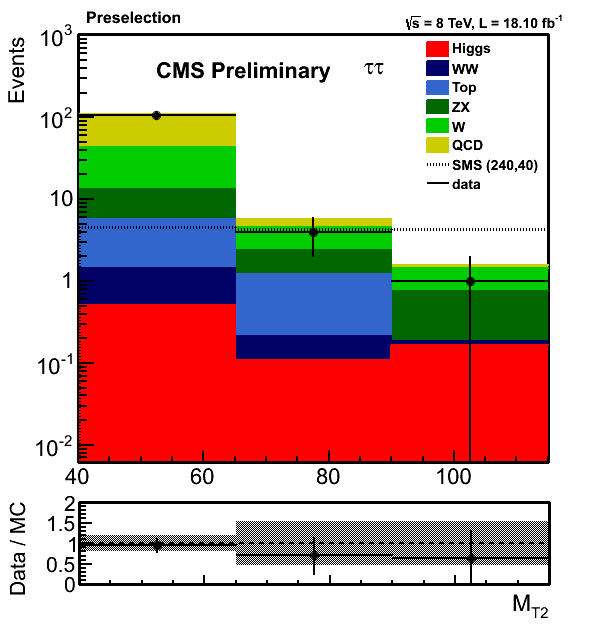
\includegraphics[width=0.35\textwidth,keepaspectratio=true]{StatisticsFig/QCDWestimation_plot.png}
%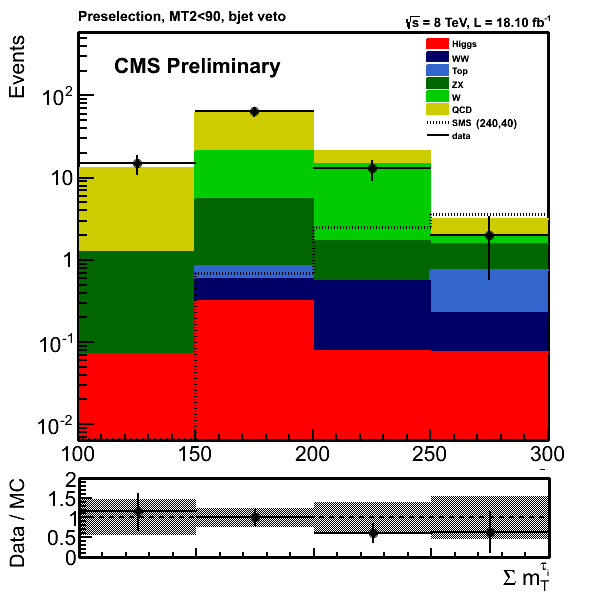
\includegraphics[width=0.35\textwidth,keepaspectratio=true]{StatisticsFig/QCDestimation_plot.png}
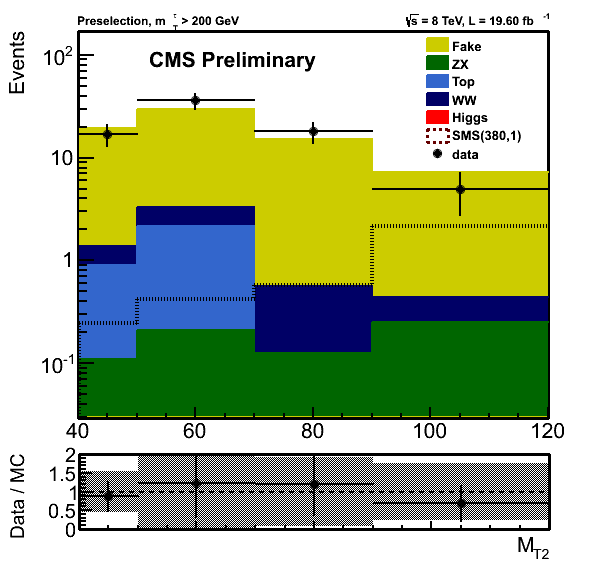
\includegraphics[width=0.35\textwidth,keepaspectratio=true]{StatisticsFig/MT2_tauMTgt200_DDFake.png}
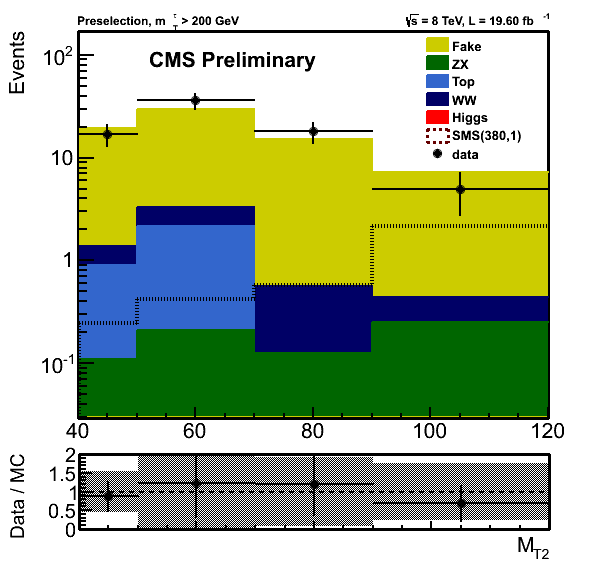
\includegraphics[width=0.35\textwidth,keepaspectratio=true]{StatisticsFig/MT2_tauMTgt200_DDFake.png}
\caption{The comparison of data and MC expectation in \leptonTau channels.}
\label{fig:yield_final}
\end{figure}
compares the data and the MC expectation in different \leptonTau channels. 
In these plots, the QCD multijet and \wjets and fake contribution from other channels is shown 
as ``Fake'' which was described in Sec.\ref{sect:bkgFake}. 
In these 2 plots, all of the statistical and systematical uncertainties are considered.
In Fig.\ref{fig:5QCDbg}, the \mttwo and \SumMT variables in two 
different signal regions of \tauTau channel are shown. The QCD multijet contribution in these plots come from the data driven method described in 
Sec.\ref{sect:bkgQCD}. The \wjets in the last bin of the top-left plot was described in Sec.\ref{sect:bkgW}. 

Backgrounds are taken into account in different categories, including Monte-Carlo-Driven, Low rate backgrounds, Fake and QCD which are data driven.
%However, due to the method of background estimation in the \tauTau channel \binone,  this channel has one more category 
%called W-jets (W).
As a summary of results, the data and background yields and systematic uncertainties are listed in Table \ref{tbl:yieldSysSummary}. 
\begin{table}[!htb]
\begin{center}
%\begin{tiny}
\caption{Data yields and background predictions with uncertainties in the four signal regions of the search. 
%The first two lines are based on Monte Carlo simulation, when for the first row, a validation against data is also done. 
%The last two rows are data driven, but the ``Fake'' for the \tauTau channel is not completely data driven.
%The uncertainties are systematic, unless when there are two parts, the first part is statistics.
The uncertainties are reported in two parts, the statistical and systematic uncertainties, respectively. 
%For \wjets in \tauTau channel, the full uncertainty is
%reported and considered as systematic for ``SM Total''.
The main backgrounds (\wjets and QCD multijet) are derived from data as described in Section~\ref{sect:bkg},
The abbreviation ``VV'' refers to diboson events.
}
\begin{tabular}{|c|c|c|c|c|}
\hline
	           & \eTau & \muTau & \tauTau \binone & \tauTau \bintwo \\
\hline
 Z+jets            & 0.19 $\pm$ 0.04 $\pm$ 0.03 & 0.25 $\pm$ 0.06  $\pm$ 0.04  &  0.56 $\pm$ 0.07 $\pm$ 0.12 & 0.81 $\pm$ 0.56 $\pm$ 0.18  \\
\ttbar, VV, hX  & 0.03 $\pm$ 0.03 $\pm$ 0.02 & 0.19 $\pm$ 0.09  $\pm$ 0.09  &  0.19 $\pm$ 0.03 $\pm$ 0.09 & 0.75 $\pm$ 0.35 $\pm$ 0.38  \\
\wjets             & 3.30 $\pm$ 3.35 $\pm$ 0.56 & 8.15 $\pm$ 4.59  $\pm$ 1.53  &  0.70 $\pm$ 0.21 $\pm$ 0.55 & 4.36 $\pm$ 1.05 $\pm$ 1.63  \\
QCD multijet       &             -              &            -                 &  0.13 $\pm$ 0.06 $\pm$ 0.21 & 1.15 $\pm$ 0.39 $\pm$ 0.74  \\
\hline
SM total           & 3.52 $\pm$ 3.35 $\pm$ 0.56 & 8.59 $\pm$ 4.59  $\pm$ 1.53  &  1.58 $\pm$ 0.23 $\pm$ 0.61 & 7.07 $\pm$ 1.30 $\pm$ 1.84  \\
\hline
\hline
Observed           &               3            &                5             &             1               & 2     \\  
\hline
\end{tabular}
\label{tbl:yieldSysSummary}
\end{center}
\end{table}

The last row of the table shows the observed data for  each individual channel.  The uncertainties are systematic, unless when there are 
two parts, the first part is statistics.
As seen in the table, the overall background yields of all categories, 
for the \eTau, \muTau, \tauTau \binone and \bintwo are  
2.96, 7.28, 1.57 and 3.14, respectively.
MC Driven backgrounds are feed to the package as a Gamma distribution with the corresponding statistical weights for each bin.
Furthermore, 25\% systematic uncertainty on MC Driven backgrounds is also considered. These systematic uncertainties are considered uncorrelated.
All systematics are taken through LogNormal distributions. For the Low rate backgrounds, a flat 50\% uncertainty is assigned.
%Systematic uncertainties for each bin of DD backgrounds are 170\%, 79\%, 50\% and 69\% respectively. 
The QCD background estimations for 
both bins of \tauTau channel use the same category of events, so the estimation in two bins are treated 100\% correlated. 
The systematic uncertainties for the fake estimation in $\ell\Tau$ channels are also 100\% correlated. 
20\% systematic uncertainty on signal yields is considered. 
Due to the large signal sample which is used, no statistical uncertainty is assigned to signal.

Since no excess of data over the background prediction is observed, 
we close our study with setting upper limits on the testing signals.
This is conducted using a modified frequentist approach, namely CLs method \cite{read:CLs}.
In this method, the test statistic $q_\mu$ 
%\cite{cowan:asymptoticCLs} 
is a function of the profile likelihood-ratio,

\begin{align}
q_\mu = -2 \ln \frac{\mathcal{L}(data ;\, b + \mu s)}{\mathcal{L}(data ;\, b + \hat{\mu} s)},
\end{align}

where $\hat\mu$ is the \textit{signal strength modifier} $\mu$ at the maximum point of the likelihood $\mathcal{L}$.
Then CLs is given by the following probability-ratio,

\begin{align}
CL_s = \frac{p(q_\mu \geq q_\mu^{obs} | b + \mu s )}{p(q_\mu \geq q_\mu^{obs} | b)}.
\end{align}
 
We compute CLs using a software package provided by the CMS Higgs PAG \cite{higgspag:software}.
After incorporating systematic uncertainties, an observed CLs smaller than 0.05 for a signal strength of $\mu = 1$, excludes the given signal at $95\%$ CL. Indeed, the package determines which signal strength $\mu$ excludes the testing signal at $95\%$ CL. Therefore all resulting $\mu \leq 1$ define the excluded region in the parameter space of the given signal. 

%To investigate the exclusion power of our research, we study the topology of direct stau pair production and the \PSGcpDo\PSGcmDo production in Simplified Models \cite{alves:sms}. 
%This research deal with tau family decay of charginoes including 
%$ \chione \rightarrow \sTau + \nu ~~\mathrm{and}~~  \chione \rightarrow \sNu_{\tau} + \tau $.
%As discussed in Section \ref{sect:introduction}, the final state is full of $\tau$ and $ \sTau \rightarrow \tau + \PSGczDo  $.
%Hence many channels could be define, due to decays of tau to electrons, muons and hadrons.    

Panels represented in figure \ref{fig:limit_bins}
%%%%%%%%%%
\begin{linenomath}
\begin{figure}[h]
\centering
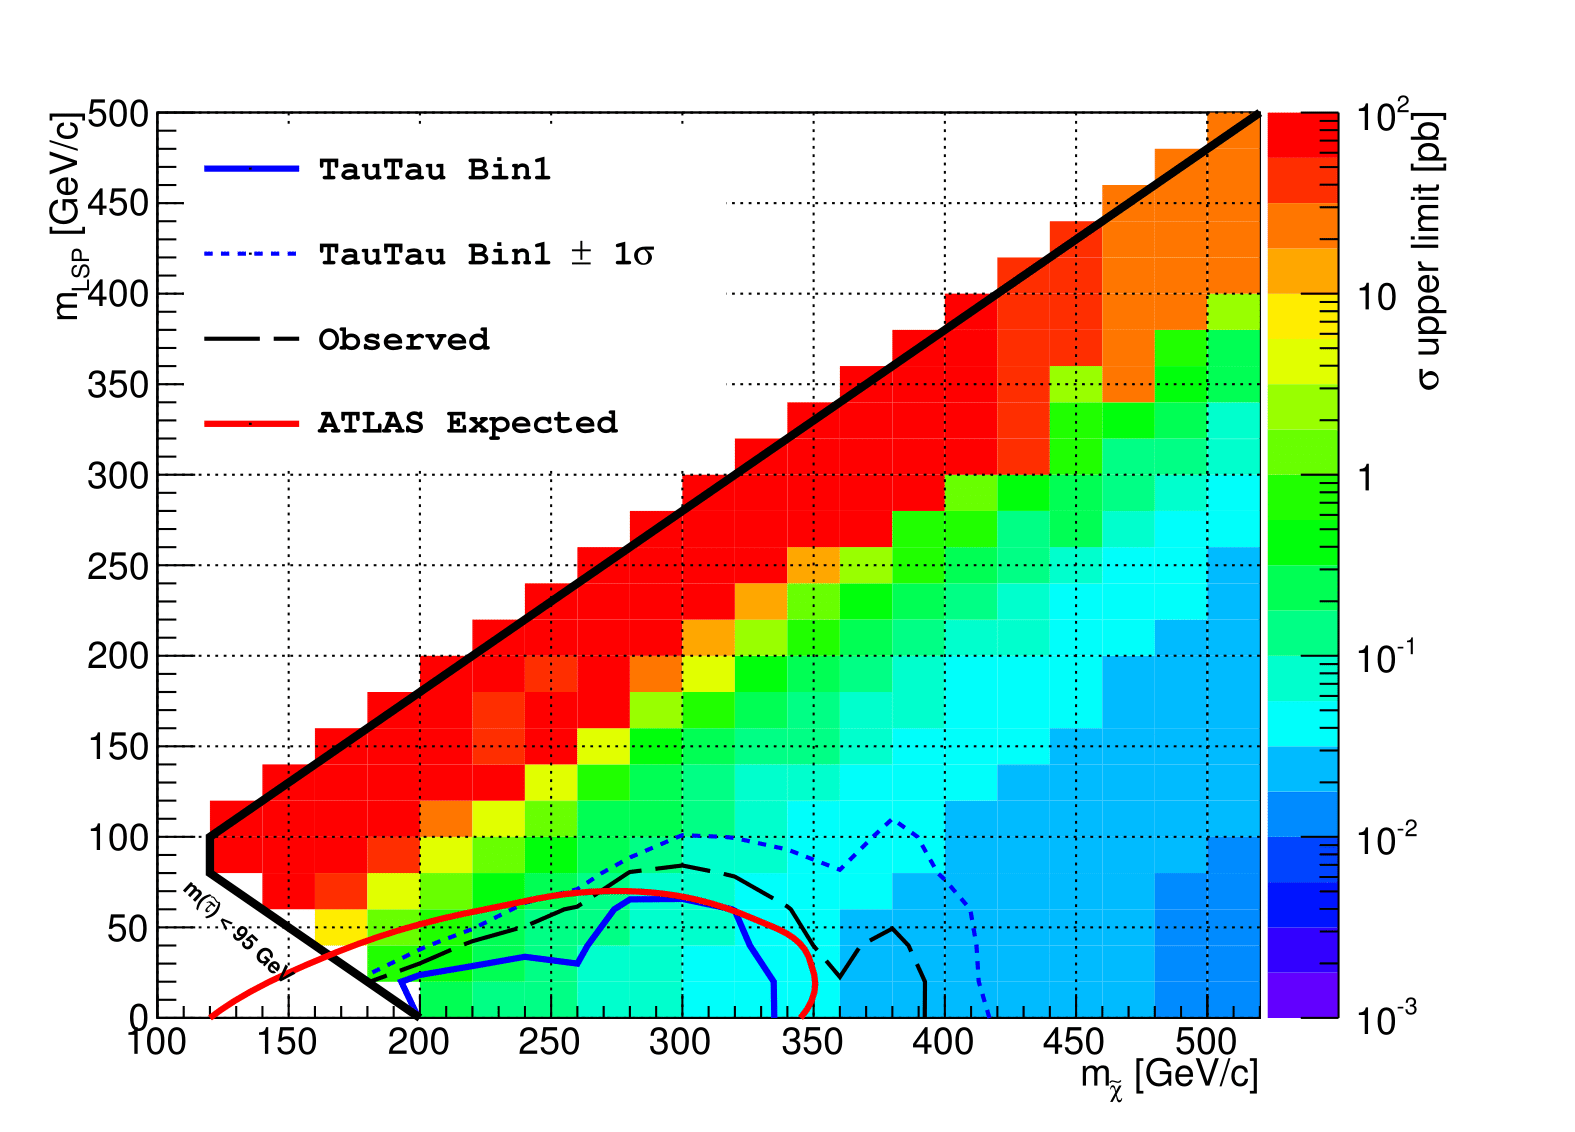
\includegraphics[width=0.49\textwidth,keepaspectratio=true]{StatisticsFig/Exclusion_TauTauBin1.png}
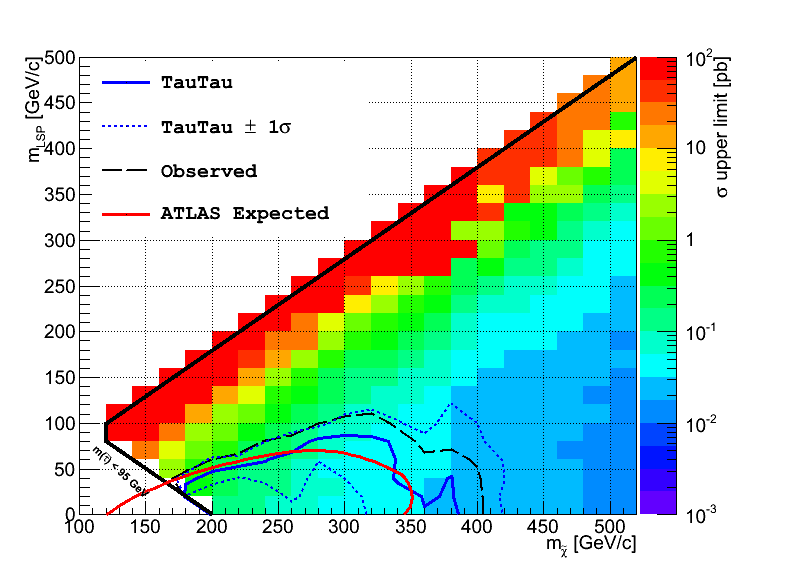
\includegraphics[width=0.49\textwidth,keepaspectratio=true]{StatisticsFig/Exclusion_TauTauBin1_Bin2.png}
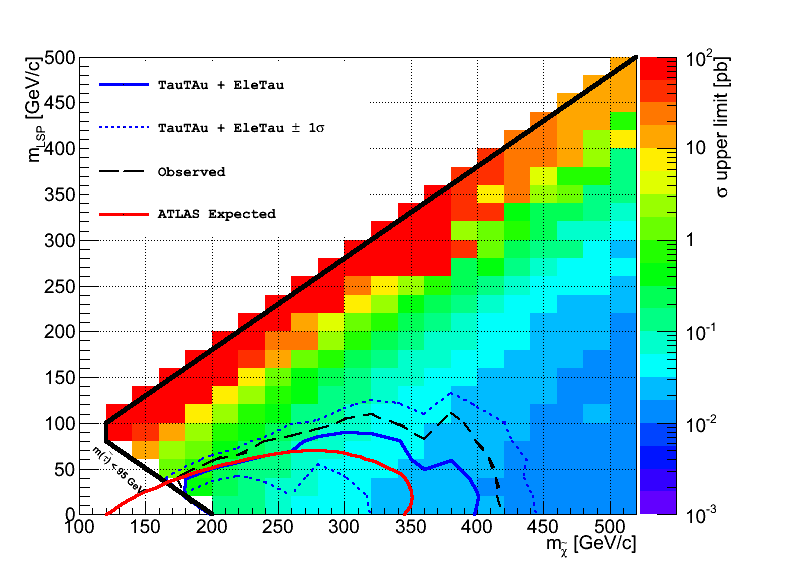
\includegraphics[width=0.49\textwidth,keepaspectratio=true]{StatisticsFig/Exclusion4Bins_MuTauExcl.png}
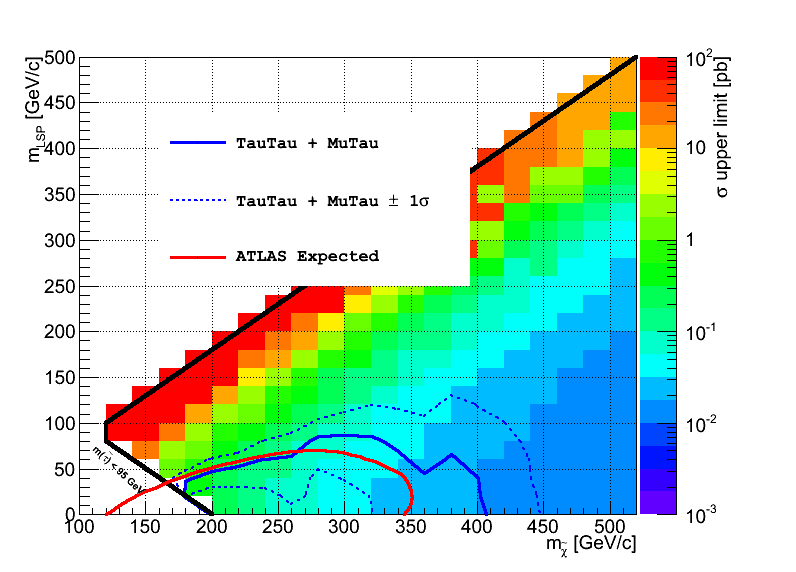
\includegraphics[width=0.49\textwidth,keepaspectratio=true]{StatisticsFig/Exclusion4Bins_EleTauExcl.png}
\caption{These figures show the impact of each bin on the final combination. 
The top panels are related to the \tauTau channel including the \binone alone (left) and combination of \binone and \bintwo (right).
The bottom ones show the expected and observed exclusion limit when \eTau (left) and \muTau (right) channels are included in the \tauTau channel.
}
\label{fig:limit_bins}
\end{figure}
\end{linenomath}
%%%%%%%%%%
 show the impact of each bin on the combined result, represented by the final exclusion limit shown in figure \ref{fig:limit_final}. 
%%%%%%%%%%
\begin{linenomath}
\begin{figure}[h]
\centering
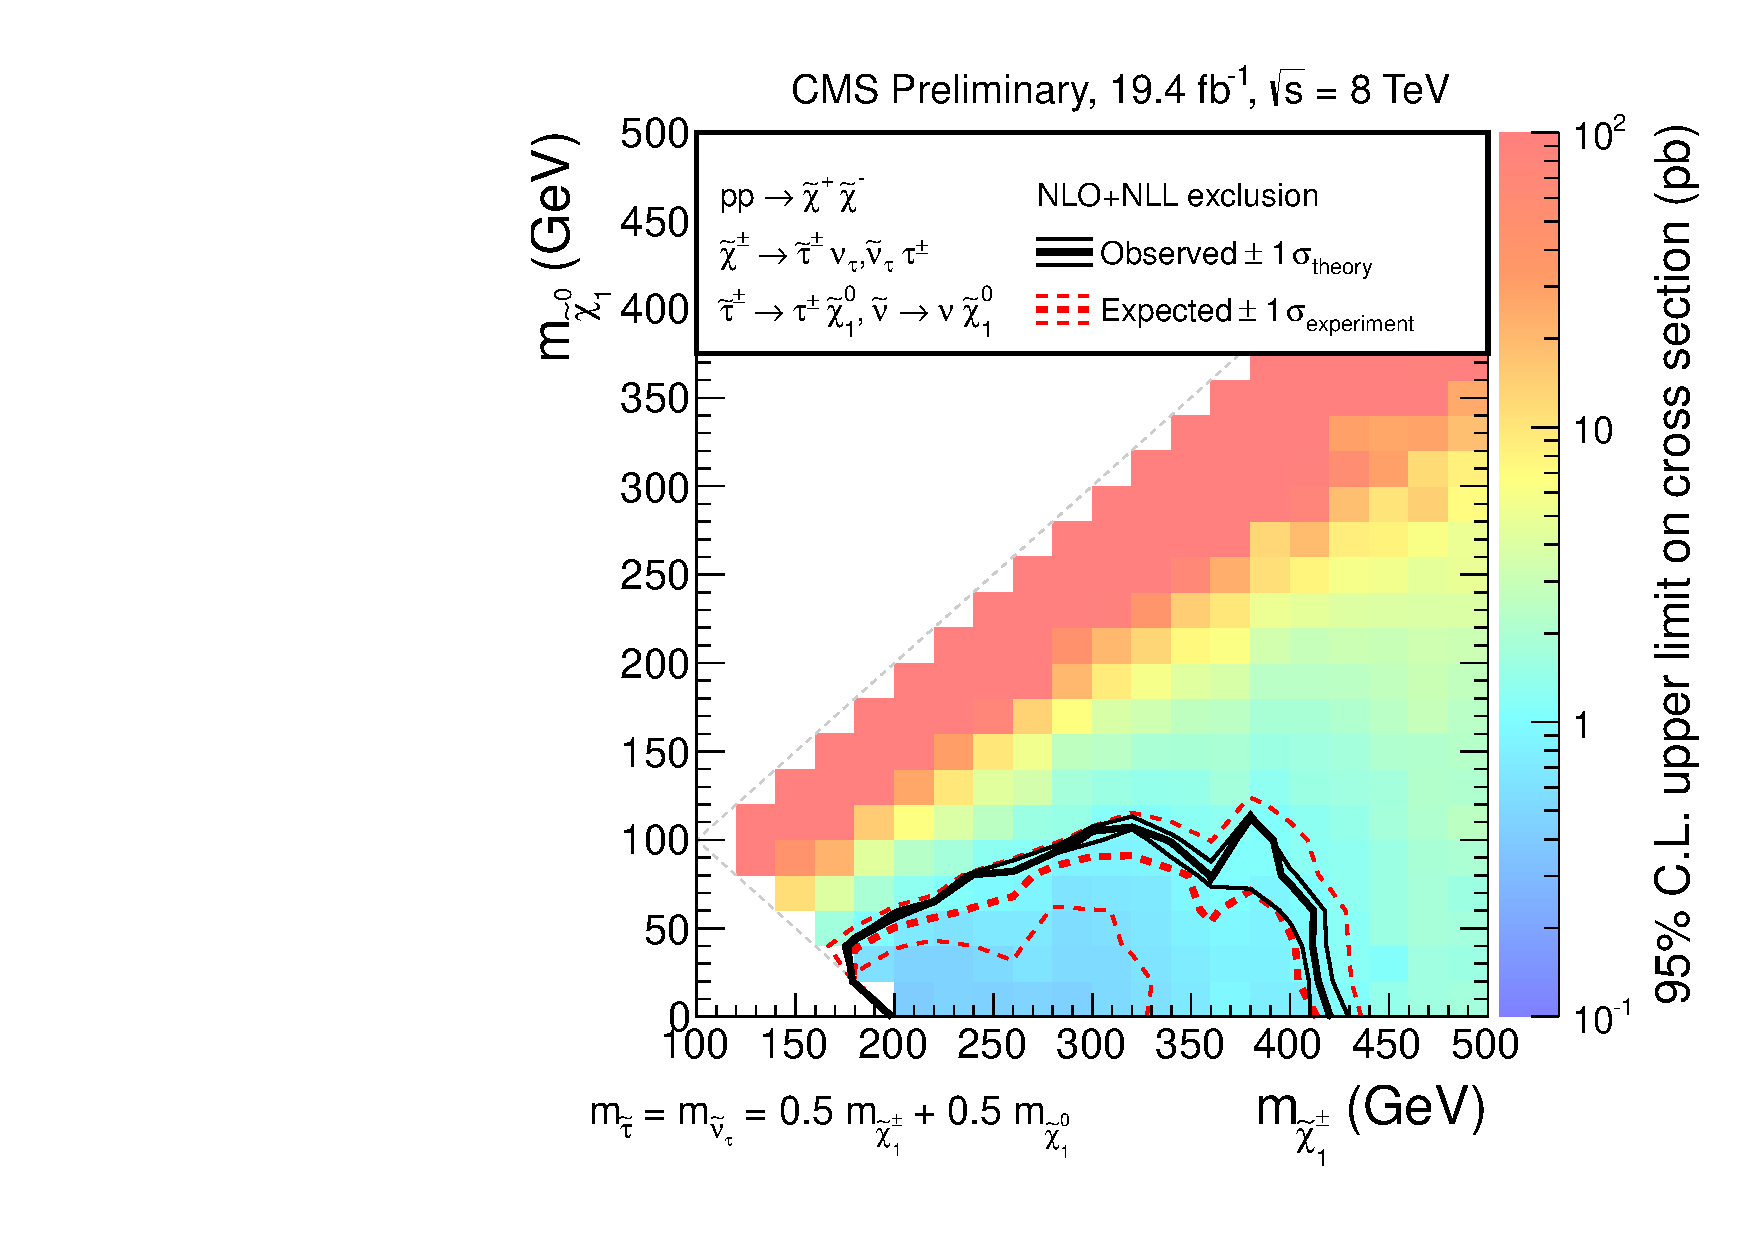
\includegraphics[width=0.7\textwidth,keepaspectratio=true]{StatisticsFig/Exclusion4Bins.pdf}
\caption{Expected exclusion power in terms of Simplified Models
with the total dataset of 2012. The observed plot is also shown.
%Backgrounds are predicted using Monte-Carlo simulations and a rough estimate of systematic uncertainties equal $10\%$ is taken into account.
}
\label{fig:limit_final}
\end{figure}
\end{linenomath}
%%%%%%%%%%
The top-left panel of figure \ref{fig:limit_bins} shows the expected and observed exclusion region in the plane of $m_{\chione}-m_{\PSGczDo}$
calculated by the simulated samples in the first bin of \tauTau channel. The top-right panel in figure \ref{fig:limit_bins} 
is produced by using both bins of \tauTau channel.
As seen, the inclusion of \bintwo of the \tauTau channel causes a little expansion of the exclusion limit towards 
the diagonal (low mass difference).
Two bottom panels of figure \ref{fig:limit_bins} show the exclusion limits when \eTau (left) and \muTau (right) channels are 
added to the \tauTau channel.  As seen, these channels individually improve the limit on the right side of plane (high mass difference).
In order to compute quickly limits, the asymptotic CLs method is used to prepare the plots of figure \ref{fig:limit_bins}.
The hybrid method is reasonably more accurate than the asymptotic method. Hence, the final exclusion limit is computed by both of the methods.
On comparison, their results were fairly the same. 
Nevertheless, the final results in figure \ref{fig:limit_final} are computed by the hybrid method.
Figure \ref{fig:limit_final} shows the expected and observed exclusion limits 
of the chargino pair production in terms of Simplified Models \cite{alves:sms}. 
Calculation of the expected exclusion limits shows that the search has a potential to exclude 
a sizable region of the phase space, surrounded by the lines of $m_{\chione} = 410\GeV$ and $m_{\PSGczDo} = 100\GeV$ with 
the total dataset of 2012. The boundaries are well beyond the ATLAS reach which is \chione  masses up to 345 \GeV \cite{Aad:2014yka}.
Adding \leptonTau channels
and considering two signal regions in \tauTau channel has increased the sensitivity of the current search compared to ATLAS which uses only 
one search region in \tauTau channel to make the exclusion.
The observed limit excludes the $\chione$ with masses up to 420 \GeV when the $\PSGczDo$ mass is zero.
The \sTau searches in the LEP experiments \cite{lepsusy} have excluded the masses below 95 \GeV. In Fig.~\ref{fig:limit_final}, 
this region corresponds to the triangle in bottom-left corner.
The diagonal line denotes the boundary for $m_{\chione} = m_{\tau} + m_{LSP}$, which is the kinematical boundary of the search.
The expected limits and their one standard deviations introduced by the experimental 
uncertainties are shown with the red solid and dashed lines, respectively. The observed limits are shown with the black solid lines, the one 
standard deviations are shown with narrower black lines. The theoretical cross sections are moved up and down by one one standard deviation to 
find the narrow lines.
The signal cross sections in NLO + next-to-the-leading-logarithm (NLL) order in $\alpha_s$ are used to make the exclusion limits.
In the whole region, the observed limits lie closer than one standard deviation from the expected limits.  



The results of the \tauTau channels are interpreted to set limit on the $\tilde{\tau}\tilde{\tau}$ production, which corresponds to the right diagram in Fig.~\ref{fig:Productions}. In this simplified model, two $\tilde{\tau}$ are directly produced from the $pp$ collision and decay instantly into two $\tau$ and two \PSGczDo. As the cross section of direct production of sleptons is lower,
\begin{linenomath}
\begin{figure}[h]
\centering
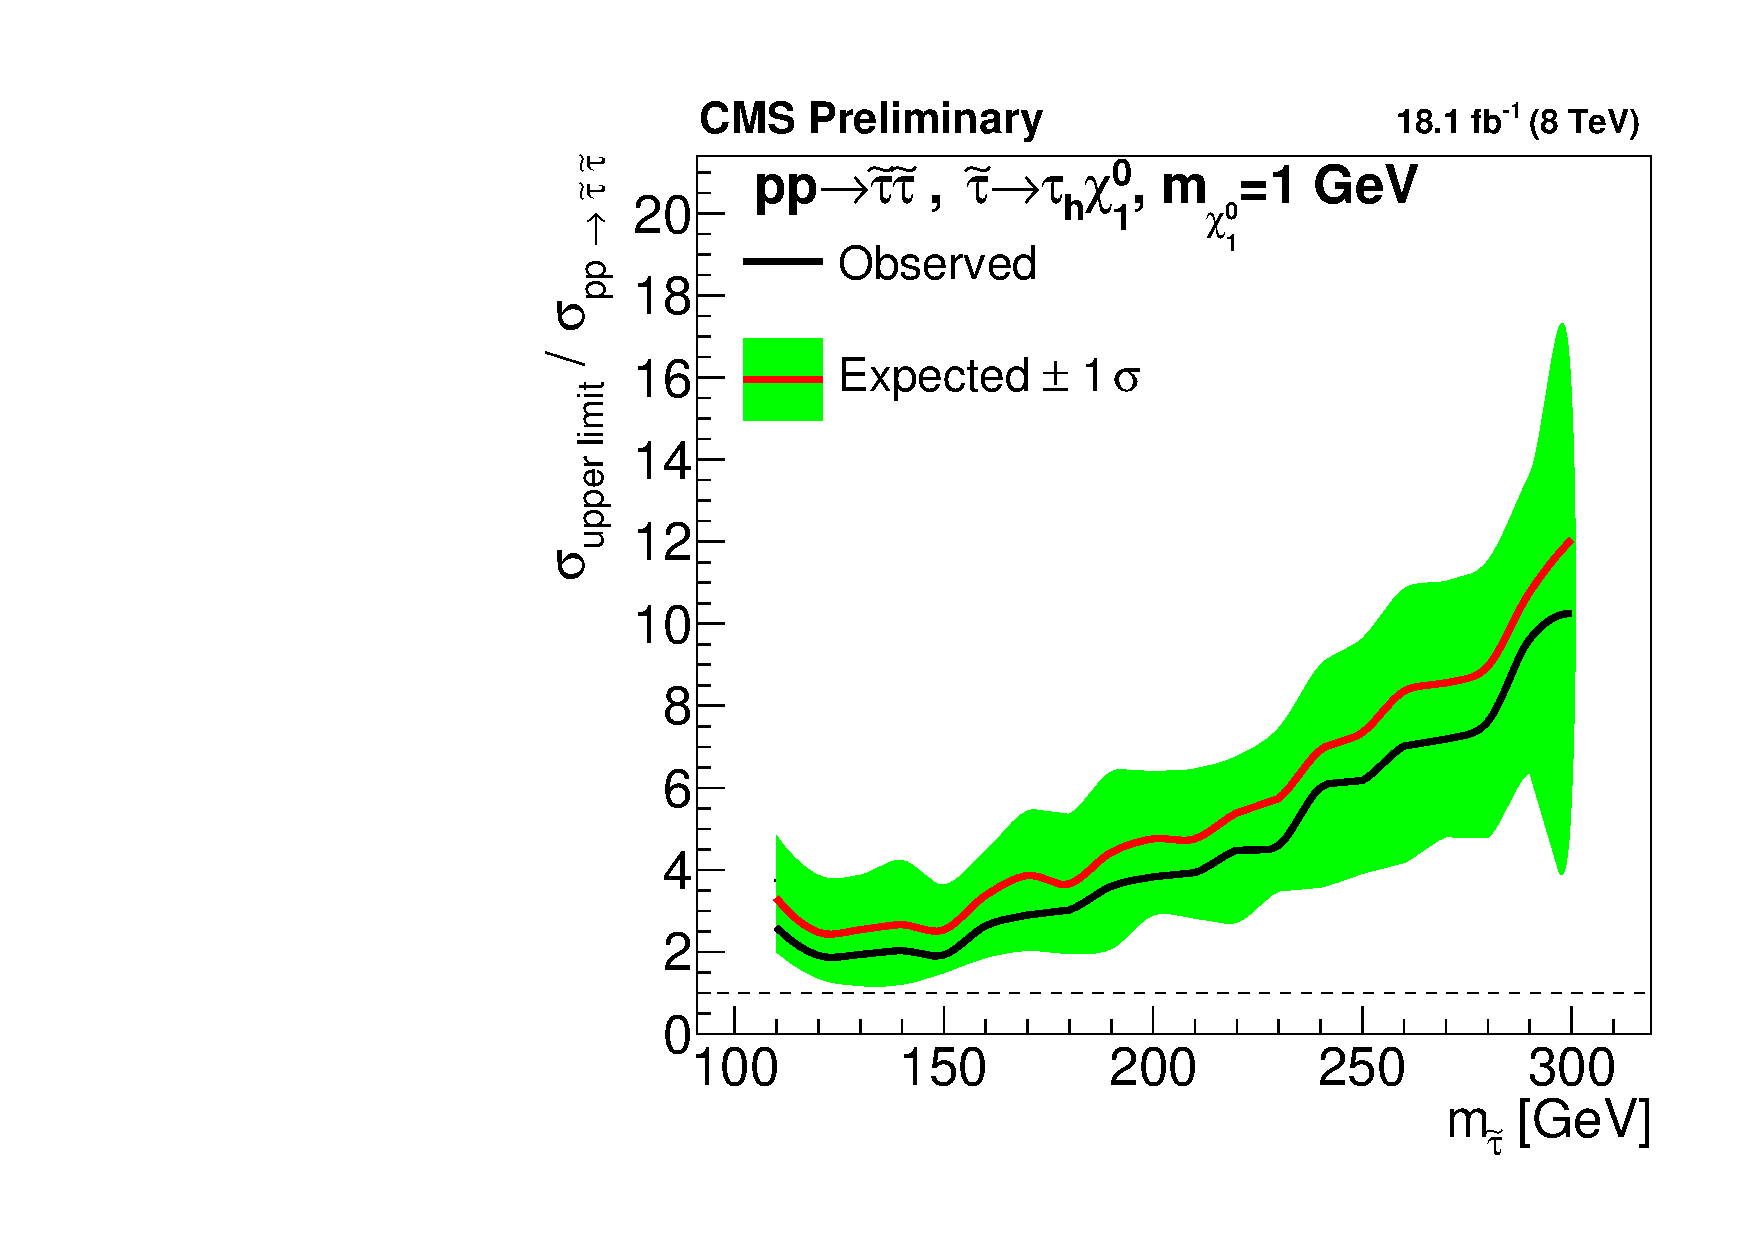
\includegraphics[width=0.5\textwidth,keepaspectratio=true]{StatisticsFig/ExclusionSTauSTauLsp1.pdf}
\caption{The exclusion power of the \tauTau channels in $\tilde{\tau}\tilde{\tau}$ production.}
\label{fig:limit_stau_stau}
\end{figure}
\end{linenomath}
 no point is excluded and $95\%$ upper limit is set on the cross section. Adding two $\ell\Tau$ channels does not improve the results.
Figure ~\ref{fig:limit_stau_stau} represents the ratio of the 
obtained upper limit on the cross section and the cross section expected from SUSY (signal strength) vs. the mass of the $\tilde{\tau}$ particle, when \PSGczDo mass is $1 GeV$.
The observed ratio is within one standard deviation of  the expected ratio.
The best limit which corresponds to the lowest signal strength is obtained for $m_{\tilde{\tau}}=110 GeV$. The observed (expected) upper limit on the cross section at this mass is 232 (289) $fb$ which is almost 3 times of the theoretical NLO cross section.
